%% Submissions for peer-review must enable line-numbering
%% using the lineno option in the \documentclass command.
%%
%% Preprints and camera-ready submissions do not need
%% line numbers, and should have this option removed.
%%
%% Please note that the line numbering option requires
%% version 1.1 or newer of the wlpeerj.cls file.

\documentclass[fleqn,10pt,lineno]{wlpeerj} % for journal submissions
% \documentclass[fleqn,10pt]{wlpeerj} % for preprint submissions

\newcommand{\cheng}[1]{\textcolor{green}{\textbf{Cheng: }{\footnotesize #1}}}
\newcommand{\alasdair}[1]{\textcolor{blue}{\textbf{Alasdair: }{\footnotesize #1}}}

\usepackage{bm} % bold math symbols
\usepackage{hyperref} % create hyperlinks
\usepackage[labelfont=bf]{caption} % figure captions
\usepackage{subcaption}
\usepackage[boxed]{algorithm2e} % provide environment and layout to write pseudo-code
\usepackage{IEEEtrantools} % more flexible formatting of equations
\usepackage{mathtools} % use DeclarePairedDelimiterXPP
\usepackage{etoolbox}
\hypersetup{
	colorlinks   = true, % Colours links instead of ugly boxes
	pdfauthor    = {Alasdair Tran and Cheng Soon Ong},
	pdftitle	 = {Combining Active Learning Suggestions},
}

\DeclareMathAlphabet{\mathcal}{OMS}{cmsy}{m}{n} % reset caligraphy font

% some convenient symbols
\DeclareMathOperator{\Beta}{Beta}
\DeclareMathOperator{\Bin}{Bin}
\DeclareMathOperator{\tr}{tr}
\newcommand{\A}{\mathpzc{A}}
\newcommand{\B}{\mathcal{B}}
\newcommand{\X}{\mathcal{X}}
\newcommand{\Y}{\mathcal{Y}}
\newcommand{\Ecal}{\mathcal{E}}
\newcommand{\Normal}{\mathcal{N}}
\newcommand{\Unlabelled}{\mathcal{U}}
\newcommand{\Labelled}{\mathcal{L}}
\newcommand{\R}{\mathcal{R}}
\newcommand*{\argmin}{\operatornamewithlimits{arg\,min}\limits}
\newcommand*{\argmax}{\operatornamewithlimits{arg\,max}\limits}
\newcommand{\MPBA}{\text{MPBA}}
\newcommand{\passive}{\text{passive}}
\newcommand{\Select}{\textsc{Select}}
\newcommand{\Update}{\textsc{Update}}
\newcommand{\bmu}{\bm{\mu}}
\newcommand{\bsigma}{\bm{\sigma}}
\newcommand{\btau}{\bm{\tau}}

% Expected value
\providecommand\given{}
\DeclarePairedDelimiterXPP\E[1]{\mathbb{E}}{[}{]}{}{
	\renewcommand\given{  \nonscript\:
		\delimsize\vert
		\nonscript\:
		\mathopen{}
		\allowbreak}
	#1
}
% Probability
\DeclarePairedDelimiterXPP\Prob[1]{\mathbb{P}}{(}{)}{}{
	\renewcommand\given{  \nonscript\:
		\delimsize\vert
		\nonscript\:
		\mathopen{}
		\allowbreak}
	#1
}

% Settings for algorithm blocks
\DontPrintSemicolon % don't display semicolons at the end of each line
\SetArgSty{textnormal} % no need to italicise
\SetKwProg{Fn}{function}{}{} % function keyword

\title{Combining Active Learning Suggestions}

\author[1]{Alasdair Tran}
\author[2]{Cheng Soon Ong}
\author[3]{Christian Wolf}
\affil[1]{Computational Media Lab, Australian National University}
\affil[2]{Machine Learning Research Group, Data61, CSIRO, Australia}
\affil[3]{Research School of Astronomy and Astrophysics, Australian National
          University}

\keywords{machine learning, astronomy, active learning, bandit, rank
          aggregation}

\begin{abstract}
Recent advances in sensors and scientific instruments have led to an increasing
use of machine learning techniques for managing the data deluge. Supervised
learning has become a widely used paradigm in many big data applications.
However,  labeled examples are required during the training phase of supervised
machine learning algorithms, and the labeling has become a  significant
bottleneck. This paper explores the use of machine learning algorithms for
identifying informative examples for labeling, the so-called active learning
setting. We  empirically compare several active learning heuristics on
benchmark UCI datasets, and focus on its  application to photometric
classification of the Sloan Digital Sky Survey. By considering each  active
learning heuristic as an expert recommendation of which example to label, we
propose to  combine them using bandit and rank aggregation algorithms. Our
results show that combining  active learning suggestions improves over each
individual heuristic (including passive  learning), and provides a promising
practical approach.

\end{abstract}

\begin{document}

\flushbottom
\maketitle
\thispagestyle{empty}

\section*{Introduction}

There are three ideas which are often used to elicit human responses---active
learning, bandits, and experimental designs. Although similar in spirit, these
ideas have different foundations which lead to different formulations. Related
to this but with literature from a different field is social choice theory,
which looks at how individual preferences are aggregated.

Active learning considers the setting where an agent interacts with its
environment to procure a training set. This contrasts with passive learning,
where the agent passively receives i.i.d.\, samples from some underlying
distribution. The environment is usually assumed to be infinite and the agent
has to choose a location to query an oracle for a label. We often assume
that there is no noise in the label, and hence there is no benefit of querying
the same point again. In many practical applications, the environment is
considered to be finite (but large). This is called pool-based active
learning.

A bandit problem is a sequential allocation problem defined by a set of
actions. The agent chooses an action at each time step and the environment
returns a reward. The aim of the agent is to maximize reward. In basic
settings, the set of actions is considered to be finite. There are three
fundamental formalization of the bandit problem, depending on the assumed
nature of the reward process: stochastic, adversarial and Markovian. In all
three settings the reward is uncertain, and hence the agent may have to play a
particular action repeatedly. The agent is compared to a static agent which has
played the best action. This difference in reward is called regret.

In contrast to active learning, experimental design considers the problem of
regression, i.e.\, where the label $y\in R$ is a real number. The problem here
is to choose a set of trials (say of size $N$) to gather enough information
about the object of interest. The goal is to maximize the information obtained
about the parameters of the model (of the object). It is often assumed that the
observations at the $N$ trials are independent. When $N$ is finite, this is
called exact design; otherwise it is called approximate or continuous design.
The environment is assumed to be infinite (e.g. $R^d$) and the observations are
scalar real variables.

\section*{Related Works}

There have been some attempts to combine active learning suggestions in the
literature.~\cite{baram04} use the EXP4 multi-armed bandit algorithm to
automate the selection process.~\cite{hsu15} study an improved version
EXP4.P, along with importance weighting to estimate the rewards using only the
training set.

In this paper, we try to be more comprehensive. In addition to the key bandit
algorithms, which includes Thompson sampling, UCB, and EXP3++, we also consider
social choice theory to make use of all information from the suggestions at
every step.

\section*{Problem Formulation}

\subsection*{Active Learning Suggestions}

Consider a standard classification setting, where we try to come up with a
hypothesis $h$ that maps the feature space $\X \subset \mathbb{R}^d$ to a
finite label space $\Y$. In pool-based active learning, we require that some
objects have already been labelled. In practice, this normally means that we
label a small random sample at the beginning. These become the labelled set
$\Labelled \subset \X \times \Y$, and the rest form the unabeled set
$\Unlabelled \subset \X$.

Now consider the problem of choosing the next example in $\Unlabelled$ for
querying. Labelling can be a very expensive task, perhaps because it requires
actual human experts to manually examine each object. Thus we want to be smart
in choosing the next example. This motivates us to come up with a rule
$r(\bm{x}; h)$ that gives each unlabelled example a score based only on their
feature vector $\bm{x}$ and the current hypothesis $h$. Coming up with a good
rule is itself a difficult problem, but there have been many attempts to derive
good heuristics. Five common ones are listed in Table~\ref{tab:heuristics}.
They roughly fall into two categories: uncertainty sampling and version space
reduction.

\begin{table}[h]
	\caption {Summary of active learning heuristics used in our experiments}
	\label{tab:heuristics}
	\centering
	\begin{tabular}{lll}
		\toprule
		{Heuristic}  &  Objective  \\
		\midrule
        Least Confidence &
			$\argmax_{x \in \Ecal}
			\left\{ \max_{y \in \Y} p(y | \bm{x}; \B) \right\}$ \\
		Highest Entropy &
			$\argmax_{x \in \Ecal} \left\{-\sum_{y \in \Y} p(y | \bm{x}; h)
            \log \big[ p(y | \bm{x}; h) \big] \right\}$
			\\[2ex]
		Smallest Margin &
			$\argmin_{x \in \Ecal} \left\{ \max_{y \in \Y} p(y | \bm{x}; h) -
            \max_{z \in \Y \setminus \{y\}} p(z | \bm{x}; h)  \right\}$
			\\[2ex]
		Smallest QBB Margin &
			$\argmin_{x \in \Ecal} \left\{ \max_{y \in \Y} p(y | \bm{x}; \B) -
            \max_{z \in \Y \setminus \{y\}} p(z | \bm{x}; \B)  \right\}$
			\\[2ex]
		Largest QBB KL &
			$\argmax_{x \in \Ecal} \left\{ \dfrac{1}{B}
               \sum_{b=1}^B D_{\mathrm{KL}}(p_b\|p_\B) \right\}$
			\\
		\bottomrule
	\end{tabular}
\end{table}

\subsubsection*{Uncertainty Sampling}

\cite{lewis94} introduce the idea of uncertainty sampling, where we select the
example whose class membership the classifier is least certain about. These
tend to be points that are near the decision boundary of the classifier.
Perhaps the simplest way to quantify uncertainty is~\cite{culotta05}'s least
confidence heuristic, where we pick the candidate whose most likely label the
classifier is most uncertain about. A second option is to calculate the entropy
\citep{shannon48}, which measures the amount of information needed to encode a
distribution. Intuitively, the closer class probabilities of an object are to
random guessing, the higher its entropy will be. This gives us the heuristic of
picking the candidate with the highest entropy. Finally we can pick the
candidate with the smallest margin, which is defined as the difference
between the two highest class probabilities \citep{scheffer01} Since the sum of
all probabilities must be 1, the smaller the margin is, the more uncertain we
are about the object's class membership.

\subsubsection*{Version Space Reduction}

Instead of focussing on the uncertainty of individual predictions, we could
instead try to constrain the size of the version space, thus allowing the
search for the optimal hypothesis to be more precise. The version space is
defined as the set of all possible hypotheses that are consistent with the
current training set. To quantify the size of this space, we can train a
committee of classifiers, $\B = \{h_1, h_2, ..., h_B\}$, and measure the
disagreement among the members about an object's class membership. Each
committee member needs to have a hypothesis that is as different from the
others as possible but that is still in the version space \citep{melville04}.
In order to have this diversity, we give each member only a subset of the
training examples. Since there might not be enough training data, we need to
use bootstrapping and select samples with replacement. Hence this method is
often called Query by Bagging (QBB).

One way to measure the level of disagreement is to calculate the margin using
the class probabilities estimated by the committee \citep{melville04}. This
looks similar to one of the uncertainty sampling heuristics, except now we
first average out the probabilities of the members before minimizing the
margin.~\cite{mccallum98} offer an alternative disagreement measure which
involves picking the candidate with the largest expected Kullback-Leibler (KL)
divergence from the average.

\subsection*{Combining Suggestions with Bandit Theory}

Out of the five heuristics discussed, how do we know which one is the optimal,
anyway? There have been some attempts in the literature to do a theoretical
analysis of them. Proofs are however scarce, and when there is one available,
they normally only work under very simple assumptions. For example,
\cite{freund97} show that the query by committee algorithm (a slight variant of
our QBB heuristics) guarantees an exponential decrease in the prediction error
with the training size, but only when there is no noise. Thus whether any of
these heuristics is guaranteed to beat random sampling is still an open
question.

To help us automatically choose the optimal heuristic, we now turn our
attention to the multi-armed bandit problem in probability theory. The
colorful name originates from the situation where a gambler stands in front of
a slot machine with $s$ levers. When pulled, each lever gives out a random
reward according to some unknown distribution. The goal of the game is to come
up with a strategy that can maximize the gambler's lifetime rewards while
minimizing the number of pulls.

Each heuristic has a different ability to identify the candidate whose
labelling information is most valuable. An appropriate reward is then the
incremental increase in the accuracy rate of a test set after the candidate is
added to the training set. We assume that the heuristic rewards are independent
of each other. This is reasonable since the theories with which we use to
derive the heuristics are mostly unrelated.

The main problem in multi-arm bandits is the trade-off between exploring random
heuristics and exploiting the best heuristic so far. There are many instances
in which we find our previously held beliefs to be completely wrong. Thus by
always exploiting, we could miss out on the optimal heuristic. On the other
hand, if we explore too much, it might take a long time to reach the desired
accuracy and the strategy ends up being no different from random sampling.

We shall compare four algorithms that address this exploration-vs-exploitation
problem.

\subsubsection*{Thompson Sampling}

The oldest of these is Thompson sampling \citep{thompson33} which solves the
trade-off from a Bayesian perspective.

Let $\rho_i$ be the reward\index{reward} of heuristic $r_i \in \R$. Observe
that even with the optimal heuristic, there are still two sources of error.
First, there could be error during the labelling process that causes the
accuracy rate to decrease. In addition, even without label noise, the
classifier trained on finite data might not be the right one, so we still
cannot score perfectly due to having a poor $h$. Conversely, a bad heuristic
might be able to pick an informative candidate due to pure luck. Thus there is
always a certain level of randomness in the reward received. We assume these
errors to be normally distributed:
	\begin{IEEEeqnarray*}{lCl}
		(\rho_i \mid \nu_i) \sim \Normal(\nu_i, \tau_i^2)
	\end{IEEEeqnarray*}

If we knew both the mean $\nu_i$ and the variance $\tau_i^2$ for all
heuristics, the problem would become trivially easy since we just need to
always use the heuristic that has the highest mean reward. In practice, we do
not know $\nu_i$, so let us assume that it itself follows a normal
distribution:
	\begin{IEEEeqnarray*}{lCl}
        \nu_i \sim \Normal(\mu_i, \sigma_i^2)
    \end{IEEEeqnarray*}

To make the problem tractable, let us assume that the variance $\tau_i^2$ is a
known constant. The goal now is to find a good algorithm that can estimate
$\mu_i$ and $\sigma_i^2$.

We start with a prior knowledge of $\mu_i$ and $\sigma_i^2$ for each heuristic
$r_i$. So long as we do not choose anything stupid, e.g.\ a zero variance, our
choice of prior should not matter too much in the long run. Since initially we
do not have any information about the performance of each heuristic, the
appropriate prior value for $\mu_i$ is $0$, i.e.\ there is no evidence (yet)
that any of the heuristics offers an improvement to the accuracy.

In each round, we draw a random sample $\nu_i'$ from the normal distribution
$\Normal(\mu_i, \sigma_i^2)$ fo reach $i$ and select heuristic $r_*$ that has
the highest sampled value of the mean reward:
    \begin{IEEEeqnarray*}{lCl}
        r_* = \argmax_{i} \nu_i'
    \end{IEEEeqnarray*}
We then use this heuristic to assign scores to the candidates. The object that
is deemed to be the most informative is then added to the training set and the
classifier is retrained. Next we use the updated hypothesis to predict the
labels of objects in the test set. Let $\delta$ be the reward observed, which
is the incremental increase in the accuracy rate on. We now have a new piece of
information that we can use to update our prior belief about the mean $\mu_*$
and the variance $\sigma_*^2$ of $r_*$. Using Bayes' theorem, we can show that
the posterior distribution of the mean reward remains normal:
	\begin{IEEEeqnarray*}{lCl}
        (\nu_* \mid \rho_* = \delta) \sim \Normal (\mu_*', {\sigma'_*}^2)
    \end{IEEEeqnarray*}
where
    \begin{IEEEeqnarray*}{lClllCl}
		\mu_*' &=& \frac{\mu_* \tau^2_* + \delta \sigma^2_*}{\sigma^2_* + \tau^2_*}
		&\qquad\qquad
        {\sigma'_*}^2 &=& \frac{\sigma^2_* \tau^2_*}{\sigma^2_* + \tau^2_*}
	\end{IEEEeqnarray*}

\subsubsection*{Upper Confidence Bounds}

Next we consider the Upper Confidence Bound (UCB) algorithms which use the
principle of ``optimism in the face of uncertainty''. In choosing which
heuristic to use, we first estimate the upper bound of the reward (i.e.\ make
an optimistic guess) and pick the one with the highest bound. If our guess
turns out to be wrong, the upper bound of the chosen heuristic will decrease,
making it less likely to get selected in the next iteration.

We shall consider two algorithms in the UCB family. They differ only in the way
the upper bound is calculated. In Optimally Confident UCB, \cite{lattimore15}
suggests that we pick the heuristic that maximizes the following upper bound:
    \begin{IEEEeqnarray*}{lCl}
		r_* = \argmax_{i} \overline{\rho_i} +
			  \sqrt{\dfrac{\alpha}{T_i(t)} \ln\Big(\dfrac{\psi n}{t}\Big)}
    \end{IEEEeqnarray*}
where $\overline{\rho_i}$ is the average of the rewards from $r_i$ that we
observe so far, $t$ is the time step, $T_i(t)$ is the number times we have
selected from heuristic $r_i$ before step $t$, and $n$ is the maximum number of
steps we are going take. There are two tunable parameters, $\alpha$ and $\psi$,
which the author suggests setting to 3 and 2, respectively.

\cite{cappe13} suggests that we instead consider the KL-divergence when finding
to upper bound. In the case of normally distributed rewards with known variance
$\sigma^2$, the chosen heuristic would be
    \begin{IEEEeqnarray*}{lCl}
		r_* = \argmax_{i} \overline{\rho_i} +
			  \sqrt{ 2 \sigma^2 \dfrac{\ln\big(T_i(t)\big)}{t} }
    \end{IEEEeqnarray*}

\subsubsection*{EXP3++}

Finally we consider \cite{seldin14}'s EXP3++ algorithm, which is shown to
perform well in both the stochastic (where each heuristic has an unknown reward
distribution) and adversarial regime (where there is no restriction on how the
sequence of rewards is generated).


\subsection*{Combining Suggestions with Social Choice Theory}

A drawback of the bandit methods is that at each iteration, we could only use
information from one particular suggestion. In addition, we also need to keep
around a test set, which is expensive and sometimes impossible to obtain in
practice. Since most suggestions require little computation, we could in fact
run all of them at the same time and then combine the rankings. This leads us
to Social Choice Theory. Originally developed by political scientists like
Nicolas de Condorcet and Jean-Charles de Borda, this field of study is
concerned with how we aggregate preferences of a group of people to determine,
for example, the winner of an election. It has the nice property that everyone
(or in our context, every active learning suggestion) has a voice.

For each heuristic $r_i$, we assign a score to every candidate like before.
From these scores, we obtain a preference ordering $R_i$. This is a binary
relation, where for any two candidates $x$ and $y$, $xR_iy$ and not $yR_ix$
mean that $x$ is strictly better $y$. That is, the heuristic $r_i$ thinks $x$
will give us more information upon labeling. If we have $s$ heuristics, we end
up with a set of $s$ orderings, $\{ R_1, R_2, \ldots, R_s \}$, which we call a
profile.

The central question in Social Choice Theory is how we can come up with a
preference aggregation rule. This is a function that maps the space of profiles
to a combined ranking $R$. The bandit algorithms, then, can be thought as a
special case where the map only considers one particular ordering in the
profile.

We shall examine three aggregation rules. In the most simple approach, Borda
count, we assign an integer point to each candidate. The lowest-ranked
candidate receives a point of 1, and each candidate receives one more point
than the candidate below. To aggregate, we simply add up all the points each
candidate receives from every heuristic. The candidate with the most points
is declared the winner and is to be labeled next.

We can think of Borda count, then, as ranking the candidate according to the
arithmetic mean. An alternative approach is to use the geometric mean
\citep{bedo14}, where instead of adding up the points, we multiple them.

The third approach we consider is the Schulze method. This method is more
computationally intensive since it requires examining all pairs of candidates.
In particular, we first compute the number of heuristics that prefer
candidate $i$ to candidate $j$. Let us call this $d(i, j)$. We then define a
path from candidate $i$ to $j$ as a sequence of candidates that starts with $i$
and ends with $j$, where, as we move along the path, the number of heuristics
that prefer the current candidate over the next candidate must be strictly decreasing.
Intuitively, the path is the rank of a subset of candidates, where $i$ is at
the top and $j$ is at the bottom.

Associated with each path is a strength $p$, which is the minimum of $d(i, j)$
for all consecutive $i$ and $j$ along the path. Our task, then, is to find the
path of the strongest strength from each candidate to every other. This problem
has a similar flavour to the problem of finding the shortest path. In fact, we
shall use a variant of the Floyd–Warshall algorithm to find the strongest path.
This is the most efficient implementation that we know of, taking quadratic
time in the number of candidates. Table \ref{tab:choice} shows how the three
algorithms work with a small example.

\begin{table}[h]
	\caption {An example of how Social Choice Theory algorithms rank four candidates
	          by aggregating three heuristics} \label{tab:choice}
	\centering
	\begin{subtable}{\linewidth}
		\centering
		\begin{tabular}{lrrrr}
			\toprule
			{Heuristic}  &  Ranking \\
			\midrule
				$r_1$ & B A C D \\
				$r_2$ & A C B D \\
				$r_3$ & B D C A \\
			\bottomrule
		\end{tabular}
		\caption{An example of how the three heuristics rank four candidates $A, B, C, D$.}
	\end{subtable}

	\begin{subtable}{\linewidth}
		\centering
		\begin{tabular}{lrrrr}
			\toprule
			{Candidate}  &  Borda count & Geometric mean \\
			\midrule
				A & $3 + 4 + 1 = 8$ & $3 * 4 * 1 = 12$ \\
				B & $4 + 2 + 4 = 10$ & $4 * 2 * 4 = 32$ \\
				C & $2 + 3 + 2 = 7$ & $2 * 3 * 2 = 12$ \\
				D & $1 + 1 + 3 = 5$ & $1 * 1 * 3 = 3$ \\
			\bottomrule
		\end{tabular}
		\caption{Aggregated ranking with Borda count and geometric mean: In both
		methods, candidate B receives the highest aggregated score.}
	\end{subtable}

	\begin{subtable}{\linewidth}
		\centering
		\begin{tabular}{lrrrr}
			\toprule
			{From / To}  & A & B & C & D \\
			\midrule
				A &   & 1 & 2 & 2 \\
				B & 2 &   & 2 & 3 \\
				C & 1 & 1 &   & 2 \\
				D & 2 & 0 & 1 &   \\
			\bottomrule
		\end{tabular}
		\caption{Aggregated ranking with Schulze method: We show the strongest
		path strengths between all pairs of candidates. Candidate B is the winner
		since $p(B, A) > p(A, B)$, $p(B, C) > p(C, B)$, and $p(B, D) > p(D, B)$}
	\end{subtable}
\end{table}


\section*{Empirical comparison}

\subsection*{Description of datasets}

We use 11 small datasets taken from the UCI Machine Learning Repository, along
with one large dataset SDSS from the astronomical domain.
Table~\ref{tab:datasets} shows the size and the number of classes in each
dataset, along with the proportion of the samples belonging to the majority
class and the maximum achievable accuracy rate.

\begin{table}[h]
	\caption {Overview of datasets} \label{tab:datasets}
	\centering
	\begin{tabular}{lrrrr}
		\toprule
		{Dataset}  & Size &  Classes & Majority & Max MPBA \\
		\midrule
        \href{https://archive.ics.uci.edu/ml/datasets/Glass+Identification}{glass}
        	& $214$ & $6$ & $33\%$ & $65\%$ \\
		\href{https://archive.ics.uci.edu/ml/datasets/Ionosphere}{ionosphere}
        	& $351$ & $2$ & $64\%$ & $89\%$ \\
        \href{https://archive.ics.uci.edu/ml/datasets/Iris}{iris}
        	& $150$ & $3$ & $33\%$ & $90\%$ \\
        \href{https://archive.ics.uci.edu/ml/datasets/MAGIC+Gamma+Telescope}{magic}
        	& $19~020$ & $2$ & $65\%$ & $84\%$ \\
        \href{https://archive.ics.uci.edu/ml/datasets/MiniBooNE+particle+identification}{miniboone}
        	& $129~596$ & $2$ & $72\%$ & $88\%$ \\
        \href{https://archive.ics.uci.edu/ml/datasets/Page+Blocks+Classification}{pageblock}
        	& $5~473$ & $5$ & $90\%$ & $79\%$ \\
		\href{https://archive.ics.uci.edu/ml/datasets/Pima+Indians+Diabetes}{pima}
        	& $733$ & $2$ & $66\%$ & $71\%$ \\
        \href{http://dx.doi.org/10.5281/zenodo.58500}{sdss}
        	& $2~801~002$ & $3$ & $61\%$ & $90\%$ \\
		\href{https://archive.ics.uci.edu/ml/datasets/Connectionist+Bench+(Sonar,+Mines+vs.+Rocks)}{sonar}
        	& $208$ & $2$ & $53\%$ & $78\%$ \\
        \href{https://archive.ics.uci.edu/ml/datasets/Statlog+(Vehicle+Silhouettes)}{vehicle}
        	& $846$ & $4$ & $26\%$ & $81\%$ \\
        \href{https://archive.ics.uci.edu/ml/datasets/Wine}{wine}
        	& $178$ & $3$ & $40\%$ & $94\%$ \\
		\href{https://archive.ics.uci.edu/ml/datasets/Breast+Cancer+Wisconsin+(Prognostic)}{wpbc}
        	& $194$ & $2$ & $76\%$ & $58\%$ \\
		\bottomrule
	\end{tabular}
\end{table}

\subsection*{Experimental Setup}
For each dataset, we build a classifier with the classes being the output. We
use a 10-fold stratified shuffled split cross validation. The stratified
strategy means that the proportion of the classes remain constant in each
split. We standardise all features to have zero mean and unit variance.
Although all examples has already been labelled, we simulate active learning by
assuming that certain examples do not have any labels. In particular, the
unlabelled pool size is 70\% of data up to a maximum of 10,000 examples. The
test pool consists of the remaining examples up to a maximum of 20,000 --- we
assume labels are available here. We use logistic regression with a Gaussian
kernel approximation and an L2 loss. In the binary case, the loss function is
\begin{IEEEeqnarray*}{lCl}
    L &=& \dfrac{1}{2} w^T w + C \sum_{i = 1}^n \ln\Big(1 + \exp(-y_i(f(X_i)^T w))\Big)
\end{IEEEeqnarray*}
where the first term is the regularisation term to ensure that the weight
vector is not too large, and $C$ is another regularisation hyperparameter which
we set to 1000. To speed up training time, we approximate the feature map of
the Gaussian kernel, transforming the raw features $X_i$ into a fixed
100-dimensional feature vector $f(X_i)$. In the multiclass case, we use the
One-vs-Rest strategy, where for every class, we build a binary classifier that
determines whether a particular example is in that class or not.

For the reward, we use the mean posterior balanced accuracy (MPBA) as the
reward. Compared to a simple accuracy rate, this measure takes into account the
class imbalance. Intuitively, we calculate the recall rate in each class and
then take the average, giving each class an equal weight. Refer to the appendix
for the MPBA derivation.

Given that there are 12 datasets, each with 16 learning curves, we need a
measure that can summarize in one number how well a particular suggestion or
policy does. Building on~\cite{baram04}'s deficiency measure, we define the
strength of an active learner or policy, relative to passive learning, as

\begin{IEEEeqnarray*}{lCl}
    \text{Strength}(h) &=&
    	1 - \dfrac{\sum_{t=1}^{n}\big(\MPBA(\max) - \MPBA(h, t)\big)}
    	{\sum_{t=1}^{n}\big(\MPBA(\max) - \MPBA(\passive, t)\big)}
\end{IEEEeqnarray*}
where $\MPBA(\max)$ is the accuracy achieved from using all labelled data in
the training set, and $\MPBA(h, t)$ is the accuracy achieved using the first
 $t$ examples selected by heuristic $h$. The summation can then be thought of as
the area between the best possible performance line and the learning curve of
$h$. The better the heuristic is, the faster it would approach this maximum
line, and thus the smaller the area. Finally, so that we can compare the
performance across datasets, we normalise the measure with the area obtained
from using just passive learning.

\section*{Discussion}

Figure \ref{fig:strengths} shows the strengths of all policies that we
consider, while Figure~\ref{fig:learning_curves} provides the learning curves
of a selected few. With the exception of the wpbc dataset, most of the policies
manage to beat passive learning. For the individual heuristics, the least
confidence seems to perform very well while being very simple to calculate.
This is consistent with have been observed in the literature. The best
performing bandit algorithm is EXP3++, and if we want to use information form
all heuristics, Borda count would be a good choice. On some datasets such as
magic and pima, Borda count does better than EXP3++, although the effect is
fairly small.

In practice, we do not have a representative test set that can be used to
compute the reward. Thus aggregation methods like Borda are are suitable than
bandit algorithms such as EXP3++ and Thompson sampling. In the absence of such a
test set, \cite{hsu15} addressed this problem by using importance weighting to
remove the bias in the accuracy on the training set. For this to work, however,
we need to let every training example and active learning suggestion have a
non-zero probability of being selected in every iteration.



\begin{figure}[tbp]
	\centering
	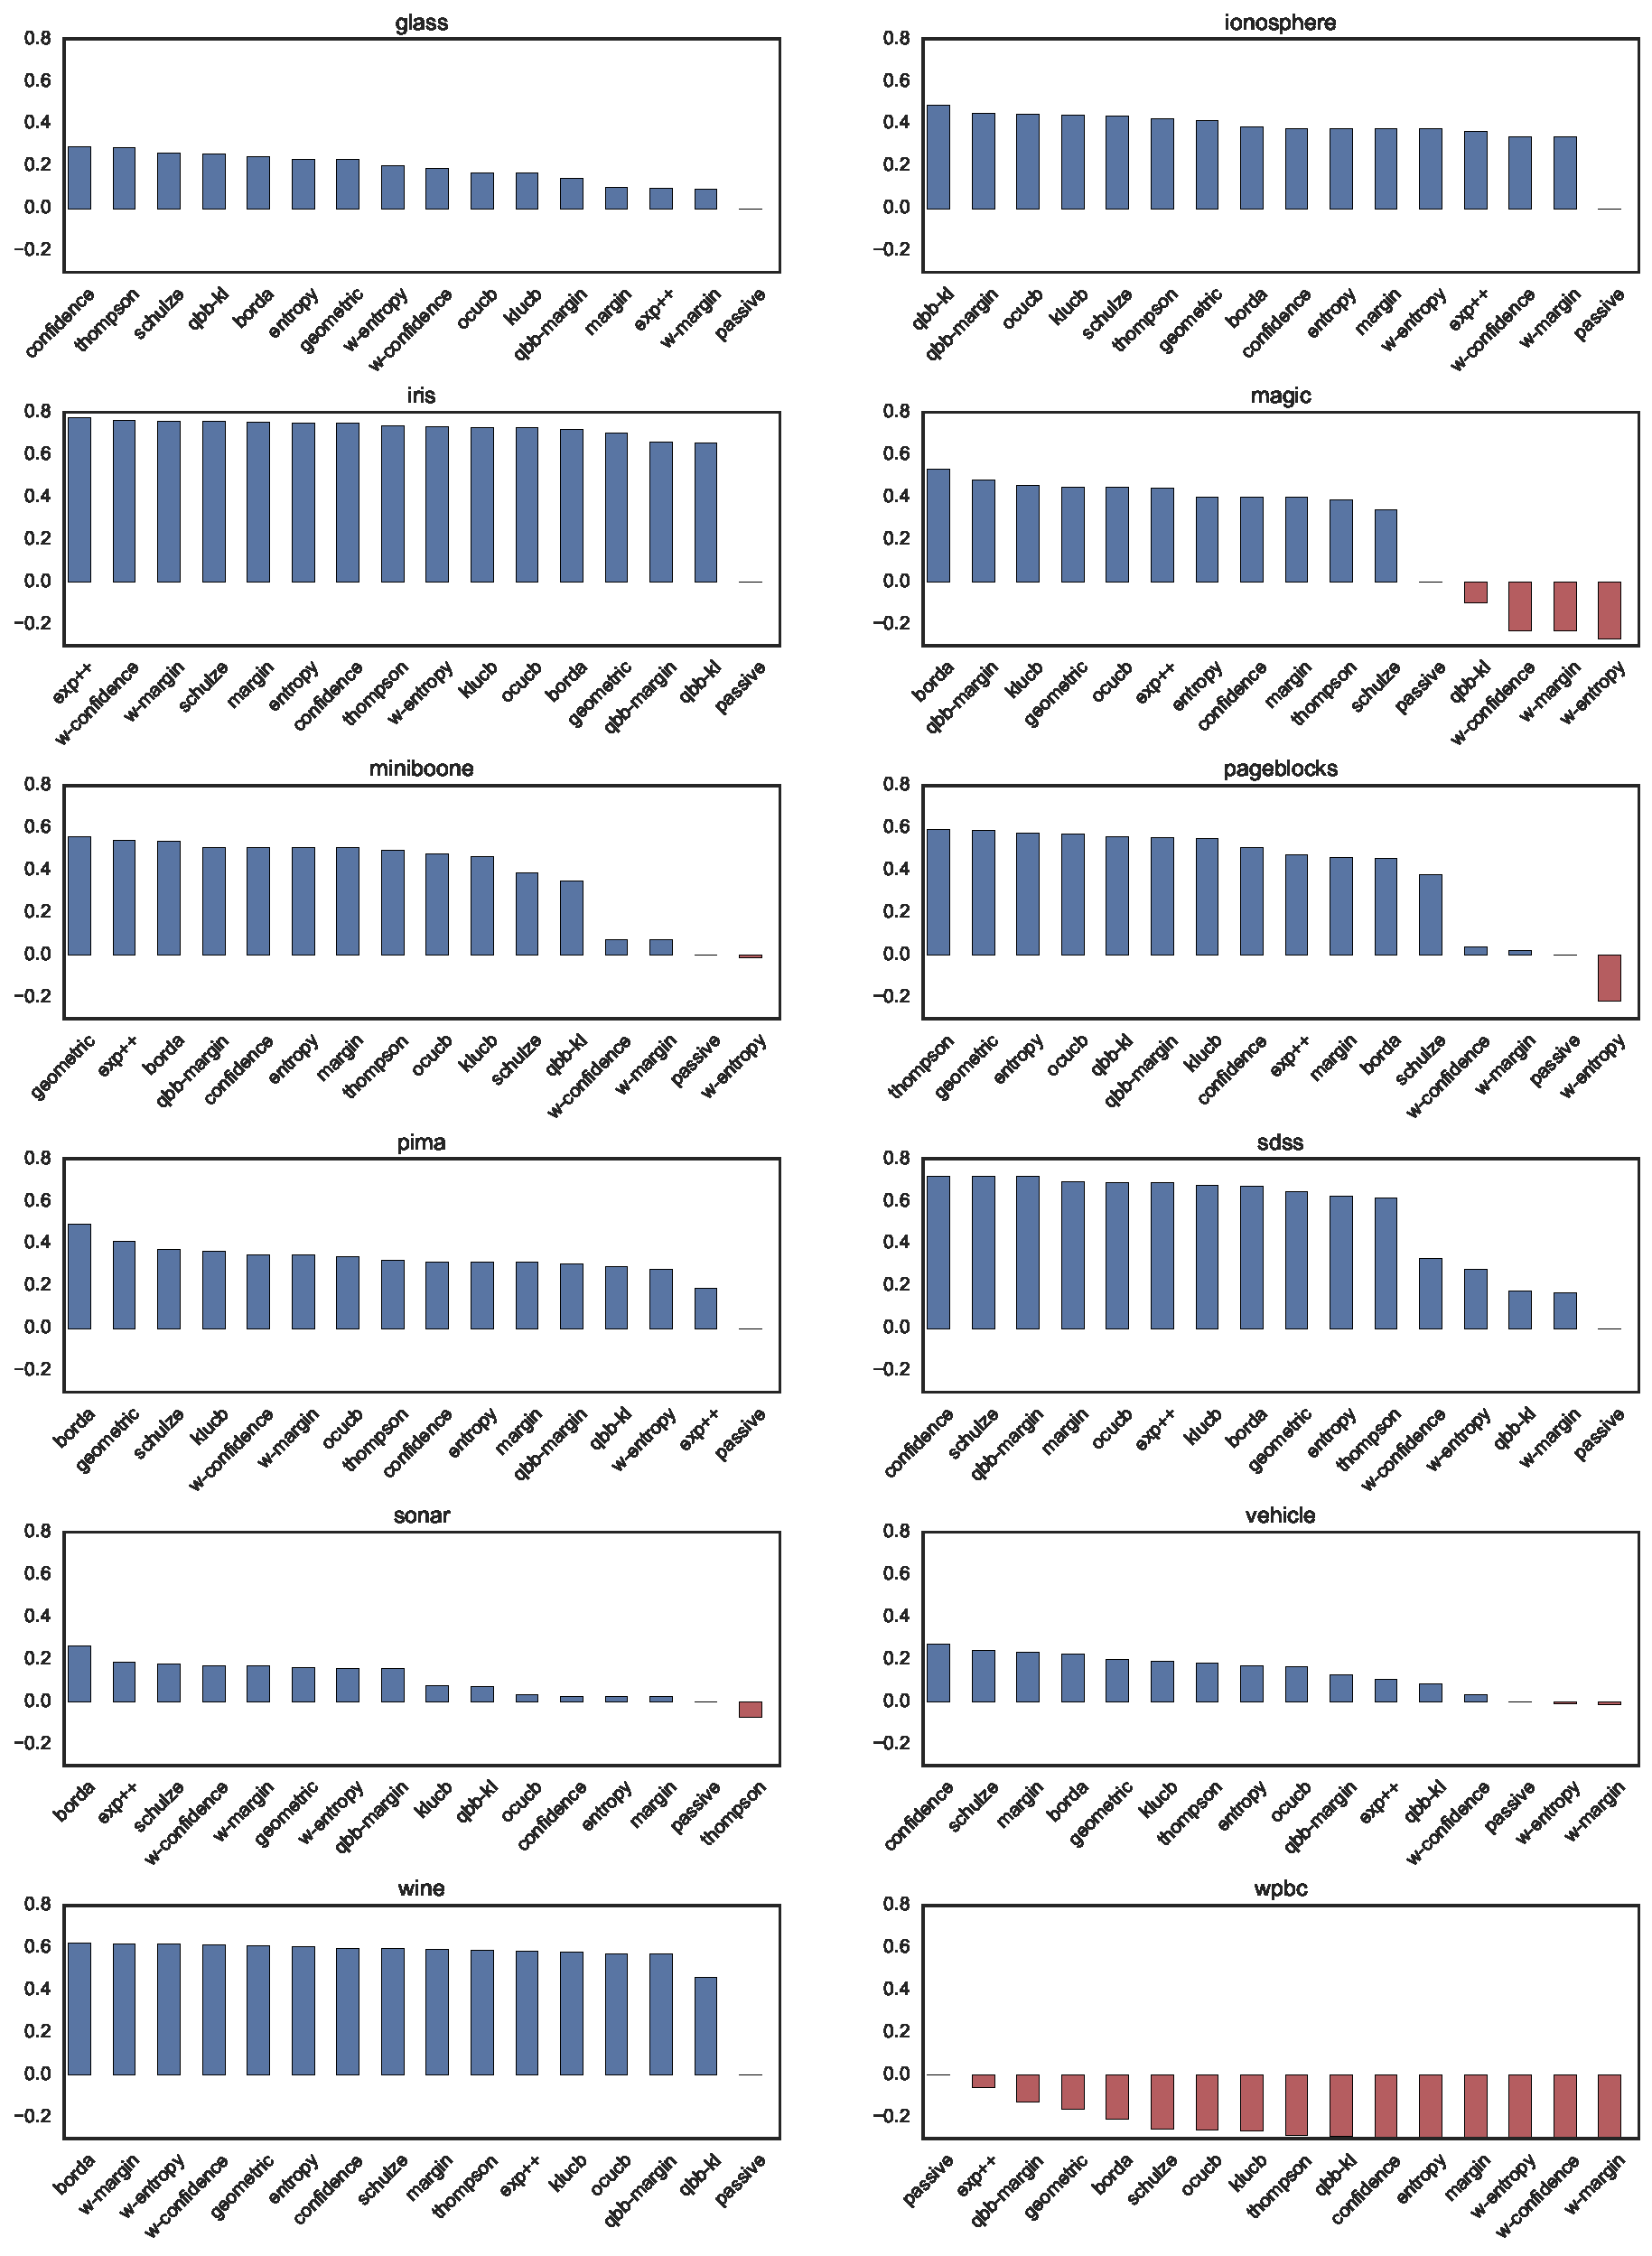
\includegraphics[width=\textwidth]{figures/strengths}
	\caption[Policy strength]{Strength of policies and heuristics relative to
	passive learning}
	\label{fig:strengths}
\end{figure}


\begin{figure}[tbp]
	\centering
	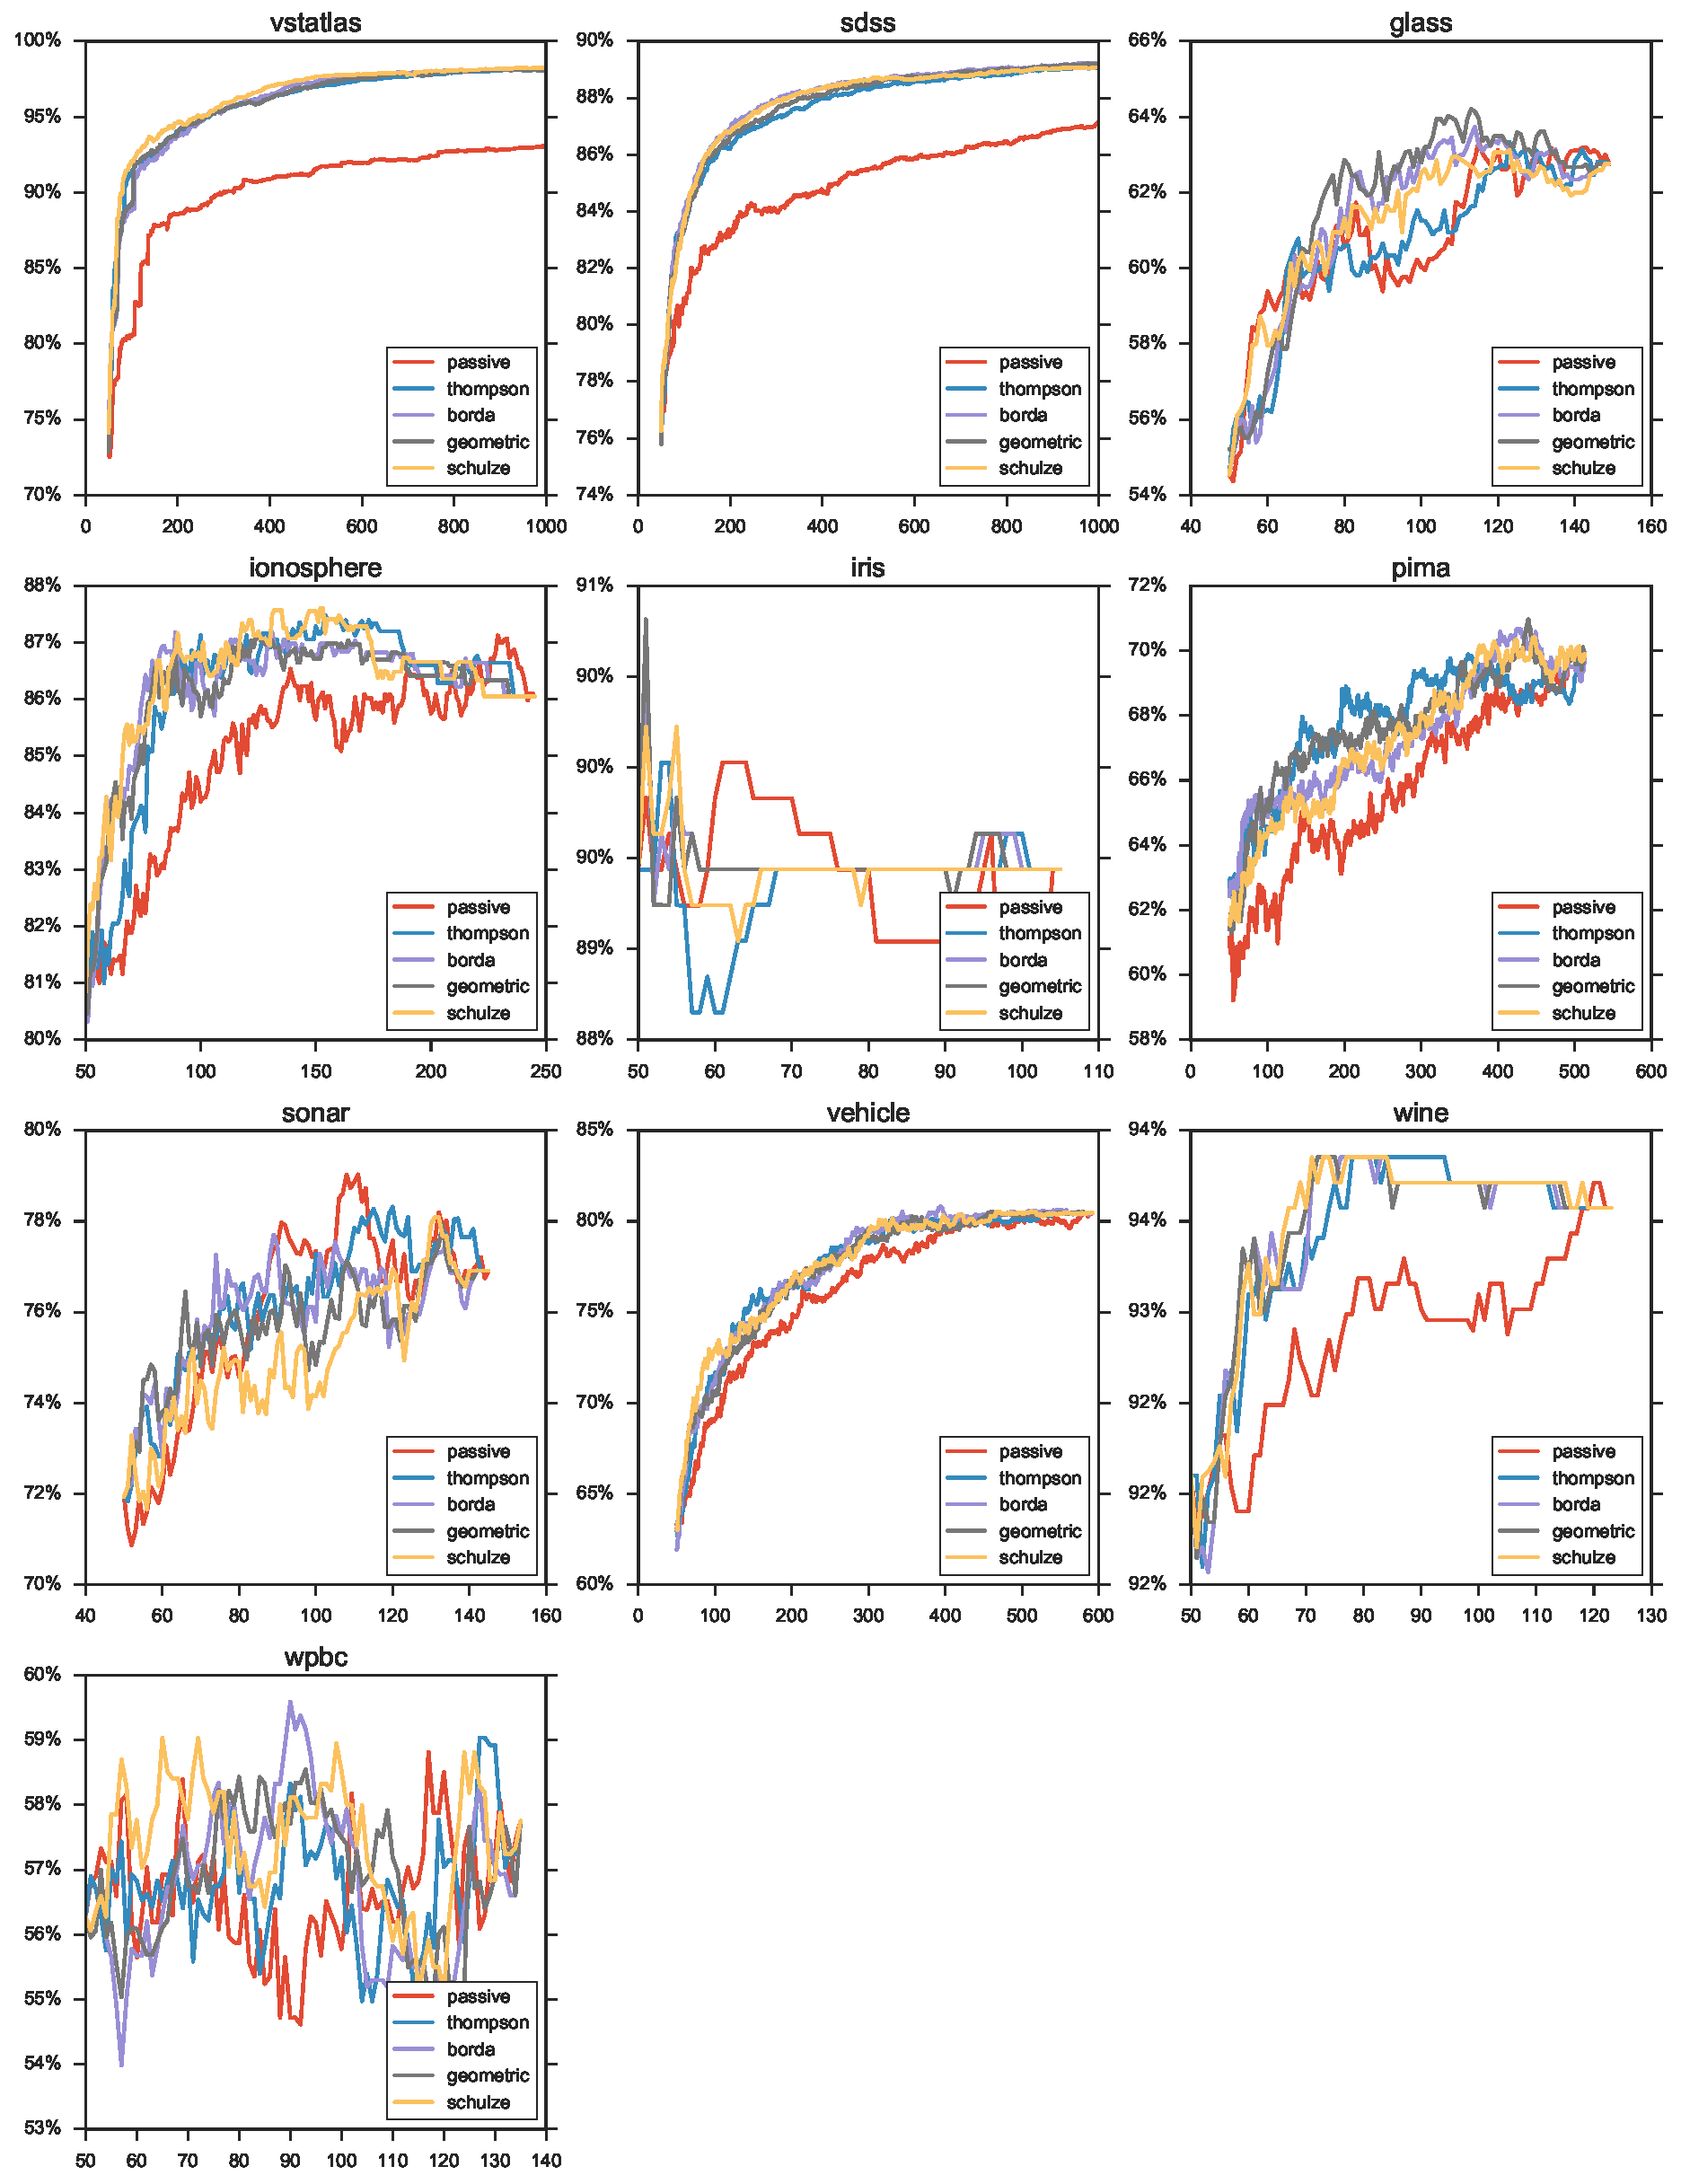
\includegraphics[width=\textwidth]{figures/learning_curves}
	\caption[Selected learning curves]{Selected learning curves. As it would
	get too cluttered to plot 16 learning curves, we only show the MPBA curves
	for the least confidence heuristic, the EXP3++ bandit policy, and the Borda
	aggregation policy.}
	\label{fig:learning_curves}
\end{figure}


\section*{Acknowledgments}

SDSS

\bibliography{active}

\pagebreak

\section*{Appendix A: Algorithms}

\begin{algorithm}[htbp]
	\KwIn{
    	unlabelled set $\Unlabelled$,
        labelled training set $\Labelled_T$,
        hypothesis $h$,
        desired training size $n$,
        query size $E$,
        set of active learning suggestions $\R$,
        and bandit algorithm $B$ with two functions \Select\,and \Update.
        }
    \BlankLine
	\While{$|\Labelled_T| < n$}{
    	Select a suggestion $r_* \in \R$ according to \Select. \;
        $\Ecal$ $\leftarrow$ random sample of size $E$ from
            $\Unlabelled$ \;
        $\bm{x}_* \leftarrow \argmax_{\bm{x} \in \Ecal} r_*
            (\bm{x})$ \;
        $y_* \leftarrow$ ask the expert to label $\bm{x}_*$ \;
        $\Labelled_T \leftarrow \Labelled_T  \cup (\bm{x}_*, y_*)$ \;
        $\Unlabelled \leftarrow \Unlabelled \setminus \bm{x}_*$ \;
        $h(\bm{x}) \leftarrow$ retrain the classifier \;
        $\delta$ $\leftarrow$ incremental increase in the accuracy \;
        Update the parameters of $B$ with \Update$(\delta)$. \;
    }
    \caption{Pool-based active learning with bandit theory}
    \label{alg:bandit}
\end{algorithm}

\begin{algorithm}[htbp]
	\KwIn{
    	unlabelled set $\Unlabelled$,
        labelled training set $\Labelled_T$,
        hypothesis $h$,
        desired training size $n$,
        query size $E$,
        set of active learning suggestions $\R$,
        and rank aggregator $G$.
        }
    \BlankLine
	\While{$|\Labelled_T| < n$}{
        $\Ecal$ $\leftarrow$ random sample of size $E$ from
            $\Unlabelled$ \;
        \For{$r \in \R$}{
        	Rank all the candidates in $\Ecal$. \;
        }
        Aggregate all the rankings into one ranking using $G$. \;
        $\bm{x}_* \leftarrow$ The highest ranked candidate in the aggregation. \;
        $y_* \leftarrow$ ask the expert to label $\bm{x}_*$ \;
        $\Labelled_T \leftarrow \Labelled_T  \cup (\bm{x}_*, y_*)$ \;
        $\Unlabelled \leftarrow \Unlabelled \setminus \bm{x}_*$ \;
        $h(\bm{x}) \leftarrow$ retrain the classifier \;
    }
    \caption{Pool-based active learning with social choice theory}
    \label{alg:bandit}
\end{algorithm}

\SetKwFunction{SelectFn}{Select}%
\begin{algorithm}[htbp]
	\KwIn{
    	set of suggestions $\R$,
        posterior mean vector $\bmu$,
        posterior variance vector $\bsigma^2$,
        likelihood variance vector $\btau^2$.
    }
    \BlankLine
    \Fn{\Select()}{
    	\For{$i \in \{1, 2, ..., |\R|\}$}{
        	$\nu_i' \leftarrow$ draw a sample from $\Normal(\mu_i, \sigma^2_i)$ \;
       	}
        $r_* \leftarrow \argmax_{i} \nu_i'$ \;
    }
    \BlankLine
    \Fn{\Update($\delta$)}{
    	$\mu_* \leftarrow \dfrac{\mu_* \tau^2_* + \delta \sigma^2_*}{\sigma^2_* + \tau^2_*}$ \;
        $\sigma_*^2 \leftarrow \dfrac{\sigma^2_* \tau^2_*}{\sigma^2_* + \tau^2_*}$ \;
    }
	\caption{Thompson sampling with normally distributed rewards}
    \label{alg:thompson}
\end{algorithm}

\begin{algorithm}[htbp]
	\KwIn{
		set of suggestions $\R$,
    	time horizon $n$,
    }
    \BlankLine
    \Fn{\Select()}{
        $r_* \leftarrow \argmax_{i} \overline{\rho_i} +
			  \sqrt{\dfrac{3}{T_i(t)} \ln\Big(\dfrac{2 n}{t}\Big)}$ \;
    }
    \BlankLine
    \Fn{\Update($\delta$)}{
		$t \leftarrow t + 1$ \;
		$T_*(t) \leftarrow T_*(t - 1) + 1$ \;
    }
	\caption{Optimally Confident UCB}
    \label{alg:oc-ucb}
\end{algorithm}

\begin{algorithm}[htbp]
	\KwIn{
		set of suggestions $\R$,
    	time horizon $n$,
    }
    \BlankLine
    \Fn{\Select()}{
        $r_* \leftarrow \argmax_{i} \overline{\rho_i} +
			  \sqrt{2 \sigma^2 \dfrac{\ln\big(T_i(t)\big)}{t}}$ \;
    }
    \BlankLine
    \Fn{\Update($\delta$)}{
		$t \leftarrow t + 1$ \;
		$T_*(t) \leftarrow T_*(t - 1) + 1$ \;
    }
	\caption{kl-UCB with normally distributed rewards}
    \label{alg:kl-ucb}
\end{algorithm}

\begin{algorithm}[htbp]
	\KwIn{
		set of suggestions $\R$,
    	time horizon $n$,
    }
    \BlankLine
    \Fn{\Select()}{
		$\beta = \dfrac{1}{2}\sqrt{\dfrac{\ln |\R|}{t |\R|}}$ \;
		$\forall i, \xi = \dfrac{18 \ln(t)^2}{t \min(1, \dfrac{1}{t} (L_i - \min(L)))^2}$ \;
		$\forall i, \epsilon = \min(\dfrac{1}{2|\R|}, \beta, \xi)  $ \;
		$\forall i, \rho = \dfrac{e^{-beta * L_i}}{\sum_j e^{-beta * L_j}}$ \;

        $r_* \leftarrow \text{draw a sample from $\R$ with probabilities $\rho$}$ \;
    }
    \BlankLine
    \Fn{\Update($\delta$)}{
		$t \leftarrow t + 1$ \;
		$T_*(t) \leftarrow T_*(t - 1) + 1$ \;
		$L_* \leftarrow \dfrac{L_* + (1 - \delta)}{(1 - \sum_j \epsilon_j)) \rho_* + \epsilon_*} $
    }
	\caption{EXP3++}
    \label{alg:exp3pp}
\end{algorithm}


\pagebreak



\section*{Appendix B: Posterior Balanced Accuracy}


Most real-world datasets are unbalanced. In the SDSS dataset, for example,
there are 4.5 times as many galaxies as quasars. The problem of class imbalance
is even more severe in the pageblock dataset, where one class makes up 90\% of
the data and the remaining four classes only make up the remaining 10\%. An
easy fix is to undersample the dominant class when creating training and test
sets. This, of course, means that the size of these sets are limited by the
size of the minority class.

When we do not want to alter the underlying class distributions or when larger
training and test sets are desired, we need a performance measure that can
correct for the class imbalance.~\cite{brodersen10} show that the posterior
balanced accuracy distribution can overcome the bias in the binary case. We now
extend this idea to the multi-class setting.

Suppose we have $k$ classes. For each class $i$ between $1$ and $k$, there are
$N_i$ objects in the universe. Given a hypothesis, we can predict the label of
every object and compare our prediction to the true label. Let $G_i$ be the
number of objects in class $i$ that are correctly predicted.
Then we define the recall $A_i$ of class $i$ as\index{recall}
	\begin{IEEEeqnarray*}{lCl}
		A_i &=& \frac{G_i}{N_i}
	\end{IEEEeqnarray*}
The problem is that it is not feasible to get the actual values of $G_i$ and
$N_i$ since that would require us to obtain the true label of every object.
Thus we need a method to estimate these quantities when we only have a sample.
Initially we have no information about $G_i$ and $N_i$, so we can assume that
each $A_i$ follows a uniform prior from 0 to 1. This is the same as a Beta
distribution with shape parameters $\alpha = \beta = 1$:
	\begin{IEEEeqnarray*}{lCl}
		A_i &\sim& \Beta(1,1)
	\end{IEEEeqnarray*}
The PDF of $A_i$ is then
    \begin{IEEEeqnarray}{lCl}
        f_{A_i}(a) &=& \frac{\Gamma(\alpha+\beta)}{\Gamma(\alpha)\Gamma(\beta)}\,
        a^{\alpha-1}(1-a)^{\beta-1} \label{eqn:prior} \\
        &\propto&   a^{1-1}(1-a)^{1-1}  \notag
    \end{IEEEeqnarray}
where $\Gamma(\alpha)$ is the gamma function.

After we have trained the classifier, suppose we have a test set containing
$n_i$ objects in class $i$. Running the classifier on this test set is the same
as conducting $k$ binomial experiments, where, in the $i$th experiment, the
sample size is $n_i$ and the probability of success is simply $A_i$. Let $g_i$
be the number of correctly labelled objects belonging to class $i$ in the test
set. Then, conditional on the accuracy rate, $g_i$ follows a binomial
distribution:
	\begin{IEEEeqnarray*}{lCl}
		(g_i \mid A_i) &\sim& \Bin(n_i, A_i)
	\end{IEEEeqnarray*}
The probability mass function of $(g_i \mid A_i = a)$ is thus
    \begin{IEEEeqnarray}{lCl}
        p_{g_i \mid A_i}(g_i) &=& \binom{n_i}{g_i} a^{g_i} (1 - a)^{n_i - g_i} \label{eqn:likelihood} \\
                              &\propto& a^{g_i} (1 - a)^{n_i - g_i} \notag
    \end{IEEEeqnarray}
In the Bayesian \index{Bayesian} setting,~\eqref{eqn:prior} is the prior and
\eqref{eqn:likelihood} is the likelihood. To get the posterior PDF, we simply
multiply the prior with the likelihood:
	\begin{IEEEeqnarray*}{lCl}
		f_{A_i \mid \bm{g}}(a)
		&\propto& f_{A_i}(a) \times f_{g_i \mid A_i}(g_i) \\
		&\propto& a^{1-1}(1-a)^{1-1} \times a^{g_i} (1 - a)^{n_i - g_i} \\
		&=& a^{1 + g_i - 1}(1-a)^{1 + n_i - g_i - 1}
	\end{IEEEeqnarray*}
Thus, with respect to the binomial likelihood function,
the Beta distribution is conjugate to itself. The posterior recall rate $A_i$
also follows a Beta distribution, now with parameters
	\begin{IEEEeqnarray*}{lCl}
		(A_i \mid g_i) &\sim& \Beta(1 + g_i, 1 + n_i - g_i)
	\end{IEEEeqnarray*}
Our goal is to have a balanced accuracy rate, $A$, that puts an equal weight in
each class. One way to achieve this is to take the average of the individual
recalls:
	\begin{IEEEeqnarray*}{lCl}
		A &=& \frac{1}{k} \sum_{i=1}^k A_i \\
		&=& \frac{1}{k} A_T
	\end{IEEEeqnarray*}
Here we have defined $A_T$ to be the sum of the individual recalls. We call
$(A \mid \bm{g})$ the posterior balanced accuracy (PBA), where $\bm{g}
=(g_1,...,g_k)$. Most of the time, we simply want to calculate its expected
value:
	\begin{IEEEeqnarray*}{lCl}
		\E{A \given \bm{g}} &=& \frac{1}{k} \, \E{A_T \given \bm{g}} \\
		&=& \frac{1}{k} \int a \cdot f_{A_T \mid \bm{g}}(a) \, da
	\end{IEEEeqnarray*}
Let us call this the mean posterior balanced accuracy (MPBA). Note that there
is no closed form solution for the PDF $f_{A_T \mid \bm{g}}(a)$. However
assuming that $A_T$ is a sum of $k$ independent Beta random variables, $f_{A_T
\mid \bm{g}}(a)$ can be approximated by numerically convolving $k$ Beta
distributions. The independence assumption is reasonable here, since there
should be little to no correlation between the individual class accuracy rates.
Knowing that a classifier is really good at recognising stars does not tell us
much about how well that classifier can recognise galaxies.

Having the knowledge of $f_{A \mid \bm{g}}(a)$ will allow us to make violin
plots, construct confidence intervals and do hypothesis tests. To get an
expression for this, let us first rewrite the cumulative distribution function
(CDF) as
	\begin{IEEEeqnarray*}{lCl}
		F_{A\mid \bm{g}}(a) &=& \Prob{A \leq a \mid \bm{g}} \\
		&=& \Prob[\Big]{\frac{1}{k} A_T \leq a \given \bm{g}} \\
		&=& \Prob{A_T \leq ka \given \bm{g}} \\
		&=& F_{A_T \mid \bm{g}}(ka) \IEEEyesnumber \label{eqn:CDF}
	\end{IEEEeqnarray*}
Differentiating \eqref{eqn:CDF} with respect to $a$, we obtain the PDF of $(A \mid \bm{g})$:
	\begin{IEEEeqnarray*}{lCl}
		f_{A \mid \bm{g}}(a) &=& \frac{\partial}{\partial a} F_{A \mid \bm{g}}(ka) \\
		&=& \frac{\partial}{\partial a} (ka) \cdot \frac{\partial}{\partial ka} F_{A_T \mid \bm{g}}(ka) \\
		&=& k \cdot f_{A_T \mid \bm{g}}(ka)
	\end{IEEEeqnarray*}

\end{document}
